\documentclass[]{article}
\usepackage[UTF8]{ctex}
\usepackage[a4paper,left=5mm,right=5mm,bottom=10mm,top=10mm]{geometry}
\usepackage{graphicx}
\usepackage{float}
\usepackage{amsmath,amsfonts,amssymb,amsthm}
\usepackage{array,color}
%opening
\title{计算机科学中的数学基础}
\author{陈昱衡 521021910939}
\date{\today}

\begin{document}

\maketitle


\section*{Warmup1}
\begin{figure}[H]
    
\includegraphics[scale = 0.8]{2023-03-29-19-26-51.png}
\end{figure}
利用二项式定理:
\begin{align}
    11^4 &= (10+1)^4\\
    &=\binom{4}{4} 10^4 + \binom{4}{3}10^3 + \binom{4}{2} 10^2 + \binom{4}{1}10 + 1\\
    &=10000 + 4000 + 600 + 40 + 1\\
    &=14641
\end{align}


\section*{Warmup2}
\begin{figure}[H]
    
\includegraphics[scale = 0.8]{2023-03-29-19-27-06.png}
\end{figure}
利用定义,我们做相邻两个二项式之商,有:
\begin{align}
    \frac{\binom{n}{k}}{\binom{n}{k-1}} &= \frac{\frac{n \times (n-1) \times \cdots (n - k + 1)}{1 \times 2 \times \cdots \times k}}{\frac{n \times (n-1) \times \cdots \times (n - k + 2)}{1 \times 2 \times \cdots \times (k-1)}}\\
    &=\frac{n-k+1}{k}\\
\end{align}
现在需要分情况讨论$n-k+1$和$k$的大小关系。\par 
于是有,
\begin{enumerate}
    \item $n$是偶数,可知,$k = \frac{n}{2}$时,有$\frac{ n - k +1}{k} \ge 1$, $k=\frac{n}{2} + 1$时,有$\frac{n-k+1}{k} \le 1$,故$\binom{n}{\frac{n}{2}} \ge \binom{n}{\frac{n}{2} - 1}$ 且$\binom{n}{\frac{n}{2}} \ge \binom{n}{\frac{n}{2} + 1}$,故此时$k = \frac{n}{2}$时$\frac{n}{k}$取最值。 
    \item $n$是奇数,可知,$k = \frac{n+1}{2}$时,有$\frac{n - k + 1}{k} = 1$,故$\binom{n}{\frac{n+1}{2}} = \binom{n}{\frac{n-1}{2}}$,故当$k = \frac{n+1}{2}$或$\frac{n-1}{2}$时,$\binom{n}{k}$取最大值。
\end{enumerate}

\section*{Warmup3}
\begin{figure}[H]
    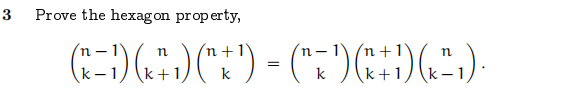
\includegraphics[scale = 0.8]{2023-03-29-19-27-19.png}
\end{figure}
按照二项式的定义将两侧的式子展开,有:
\begin{align}
    &\binom{n-1}{k-1}\binom{n}{k+1}\binom{n+1}{k} \\
    &= \frac{(n-1) \times (n -2) \times \cdots \times (n-k+1) \times n \times (n-1) \times \cdots \times (n-k) \times (n+1) \times n \times \cdots \times (n - k + 2)}{(k-1)\times (k-2) \times \cdots \times 1 \times (k+1) \times k \times \cdots \times 1 \times k \times (k-1) \times \cdots 1}\\
    &= \frac{(n-1) \times (n -2) \times \cdots \times (n-k+1) \times n \times (n-1) \times \cdots \times (n-k+2)(n-k+1)(n-k) \times (n+1) \times n \times \cdots \times (n - k + 2)}{(k-1)\times (k-2) \times \cdots \times 1 \times (k+1) \times k \times \cdots \times 1 \times k \times (k-1) \times \cdots 1}
    \\
    &=\frac{(n-1) \times (n -2) \times \cdots \times (n-k+1)(n-k) \times n \times (n-1) \times \cdots \times (n-k+2)\times (n+1) \times n \times \cdots \times (n - k + 2)(n-k+1)}{(k-1)\times (k-2) \times \cdots \times 1 \times (k+1) \times k \times \cdots \times 1 \times k \times (k-1) \times \cdots 1}
    & = \binom{n-1}{k} \binom{n+1}{k+1} \binom{n}{k-1}
\end{align}
只需将分母中的三个项稍微调整顺序即可


\section*{Warmup4}
\begin{figure}[H]
    
\includegraphics[scale = 0.8]{2023-03-29-19-27-32.png}
\end{figure}
根据对整数域二项式的定义,有
\begin{align}
    \binom{-1}{k} &= \frac{(-1)^k}{k!}\\
    &=\frac{(-1) \times (-2) \cdots \times (-k)}{k! }\\
    &=(-1)^k \times \frac{k(k-1) \times \cdots \times  2\times  1}{k!}\\
    &=(-1)^k \text {\quad  $ k \ge 0$}
\end{align}

\end{document}